% !TeX encoding = UTF-8
% !TeX spellcheck = de_DE
% !TeX program = lualatex
% !TeX BIB program = biber
%other magic comments: see TeXstudio user manual, chapter 4.10
\documentclass{standalone}

\usepackage{tikz}
\usetikzlibrary{circuits.ee.IEC}
\usetikzlibrary{circuits.logic.US}

\title{Dreiwegeweiche}
\author{Wolfgang~Witt}
\date{\today}

\begin{document}
	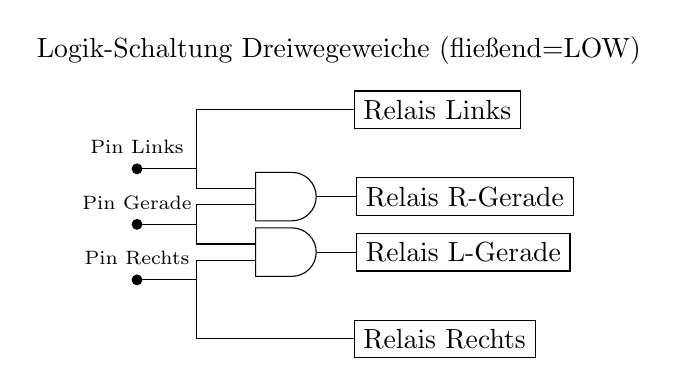
\begin{tikzpicture}[circuit ee IEC, circuit logic US, every info/.style={font=\scriptsize}]
		\node (andL) [and gate, inputs={nn}] {};
		\draw (andL.output) to ++(.5, 0) node [rectangle, draw, anchor=west] {Relais R-Gerade};
		\draw (andL.input 1) to ++(-.75, 0) to ++(0, .25) node (splitL) {} to ++(-.75, 0) node (pinL) [contact, info={Pin Links}] {};
		\draw (splitL.center) to ++(0, .75) to ++(2, 0) node (RelaisL) [rectangle, draw, anchor=west] {Relais Links};
		\draw (andL.input 2) to ++(-.75, 0) to ++(0, -.25) node (splitG) {} to ++(-.75, 0) node (pinG) [contact, info={Pin Gerade}] {};
		\draw (splitG.center) to ++(0, -.25) to ++(.75, 0) node (andR) [and gate, inputs={nn}, anchor=input 1] {};
		\draw (andR.output) to ++(.5, 0) node [rectangle, draw, anchor=west] {Relais L-Gerade};
		\draw (andR.input 2) to ++(-.75, 0) to ++(0, -.25) node (splitR) {} to ++(-.75, 0) node (pinR) [contact, info={Pin Rechts}] {};
		\draw (splitR.center) to ++(0, -.75) to ++(2, 0) node [rectangle, draw, anchor=west] {Relais Rechts};
		%Überschrift
		\path (RelaisL) ++(-1.25, .75) node {Logik-Schaltung Dreiwegeweiche (fließend=LOW)};
	\end{tikzpicture}
\end{document}
